% Neuroloop utilities - Channel tool user guide - Top level
% Written by Christopher Thomas.

\documentclass[letterpaper,11pt]{report}
\usepackage[letterpaper]{geometry}
\usepackage{graphicx}
\usepackage{verbatim}
\usepackage{placeins}
\usepackage{longtable}

\geometry{nohead,footskip=0.3in,margin=0.75in}

% Force my paragraph style, darnit.
\usepackage{indentfirst}
\setlength{\parskip}{\baselineskip}

% NOTE - "\thispagestyle" is used for part and chapter beginning pages, and
% overrides \pagestyle. Redefine it to be harmless.
% NOTE - The canonical solution ("\pagenumbering{gobble}") resets the page
% counter whenever it's used.
\renewcommand{\thispagestyle}[1]{}

% Custom macros.
\newcommand{\fixme}[1]{\textbf{FIXME: #1}}

\newcommand{\figdef}[3]
{\begin{figure}[htb]
\begin{center}#1\end{center}
\caption{#2}\label{#3}\end{figure}}

\newcommand{\tabdef}[3]
{\begin{table}[hb]
\begin{center}#1\end{center}
\caption{#2}\label{#3}\end{table}}

% Document body.
\begin{document}
%
% Title page.
%
\pagestyle{empty}

\begin{center}
%
\vspace*{1in}
{\Huge NeuroLoop Channel Tool -- User Guide} \\
{\footnotesize Written by Christopher Thomas -- \today.}
%
\vspace*{1.5in}\\
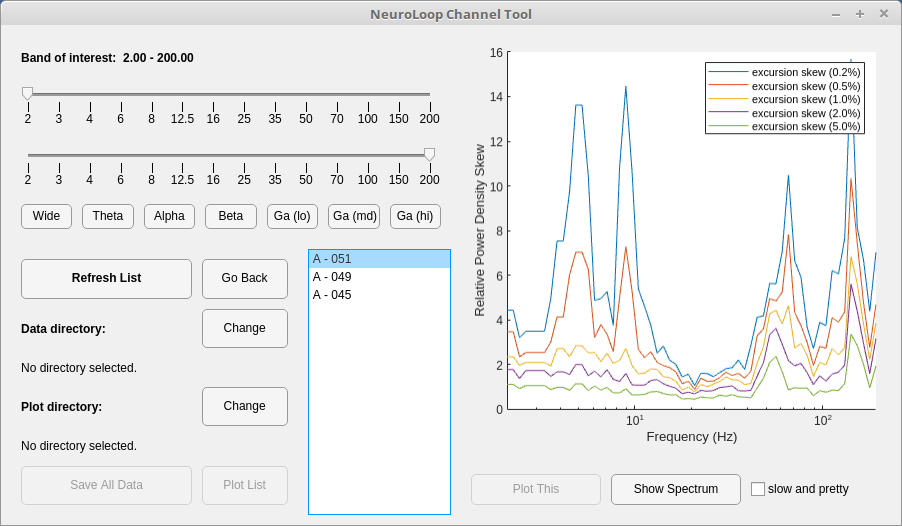
\includegraphics[width=5in]{screenshots/20201013/gui-4c-burst-chanexcursion}
%
\end{center}
%
\vfill
{\tiny \input{../LICENSE.md}}
%
\clearpage
%
%
% Front matter.
%
\pagestyle{plain}
\pagenumbering{roman}
\setcounter{page}{1}
%
\tableofcontents
%
\clearpage
%
%
% Document parts.
%
\pagestyle{plain}
\setcounter{page}{1}
\pagenumbering{arabic}
%
% Neuroloop utilities - Channel tool user guide - Overview
% Written by Christopher Thomas.

\chapter{Overview}
\label{sect-over}

The ``NeuroLoop Channel Tool'' is a GUI application that looks at folders
containing neural recordings and identifies channels that have spikes and
channels that have LFP bursts.

The intended use of this tool is for examining high-channel-count recordings
to identify channels that have interesting behavior without a human having
to manually examine each channel. The tool is designed to do this quickly
enough that it may be used during experiments (analyzing a short initial
recording to identify channels of interest in the primary experiment).

Chapter \ref{sect-howto} gives a walk-through of how to use the Channel Tool.

\fixme{Stub content.}

%
% This is the end of the file.

% Neuroloop utilities - Channel tool user guide - How-To
% Written by Christopher Thomas.

\chapter{Walk-Through}
\label{sect-howto}

%
%
\section{Installation}
\label{sect-howto-install}

The NeuroLoop Channel Tool consists of a single Matlab script
(\verb|nloop_channeltool.m|) that makes use of the NeuroLoop utility
libraries.

To install the tool, first make sure that the NeuroLoop utility libraries
are on path, then make sure that the Channel Tool script is on path, and
finally type ``\verb|nloop_channeltool|'' in Matlab to launch the tool.

%
%
\section{Data Selection Screen}
\label{sect-howto-select}

When the Channel Tool is launched, it shows the data selection dialog
(Figure \ref{fig-howto-select-1}). To use this dialog:
\begin{itemize}
\item Click the ``Select Data Directory'' button. This brings up a file
browser window.
\item Navigate to the directory containing your data.
\item Click ``open'' in the file browser window.
\end{itemize}

\figdef{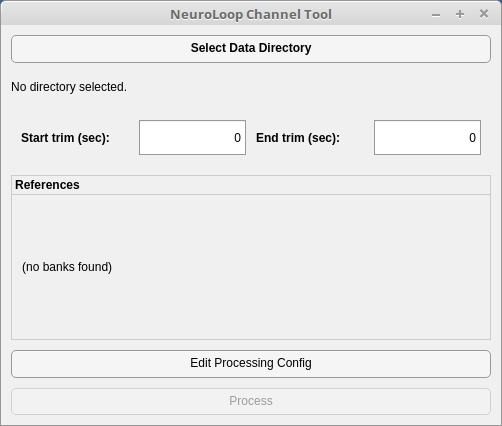
\includegraphics[height=3in]{screenshots/20201013/gui-1a-select}}
{Data selection dialog on startup.}{fig-howto-select-1}

After selecting a directory, the Channel Tool will attempt to read metadata.
If successful, it will enable reference selection and processing
(Figure \ref{fig-howto-select-2}).
\textbf{Make sure to finish configuration before clicking ``process'':}
\begin{itemize}
\item For each detected bank of channels, select a channel in that bank to
use as the reference. This removes common-mode noise from the channels.
\item If there are known artifacts at the beginning or end of the signal,
edit the ``trim'' times to remove the specified number of seconds from the
start and end.
\item If you want to adjust the settings used when loading and filtering the
data, click the ``Edit Processing Config'' button.
\item \textbf{After all of that is done}, click ``Process''.
\end{itemize}
You can go back to the setup dialog later to adjust configuration and re-read
the data (or to read a different data set). The problem is that loading and
filtering the data takes a long time, so you only want to do it when it's
necessary.

\figdef{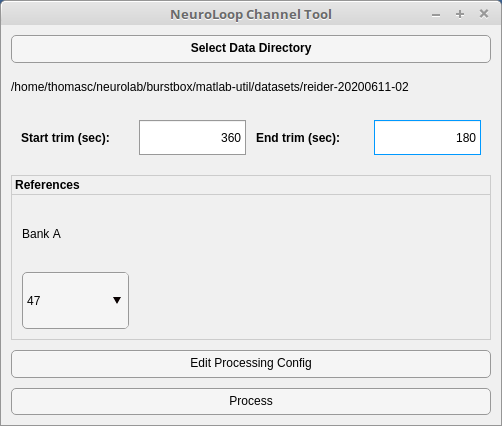
\includegraphics[height=3in]
{screenshots/20201013/gui-1b-select-filled}}
{Data selection dialog after choosing a directory.}{fig-howto-select-2}

%
%
\clearpage
\section{Processing Configuration Dialog}
\label{sect-howto-procconfig}

The processing configuration dialog (Figure \ref{fig-howto-procconfig}) lets
you adjust the filtering and artifact-rejection settings used when loading
and processing channels.

\figdef{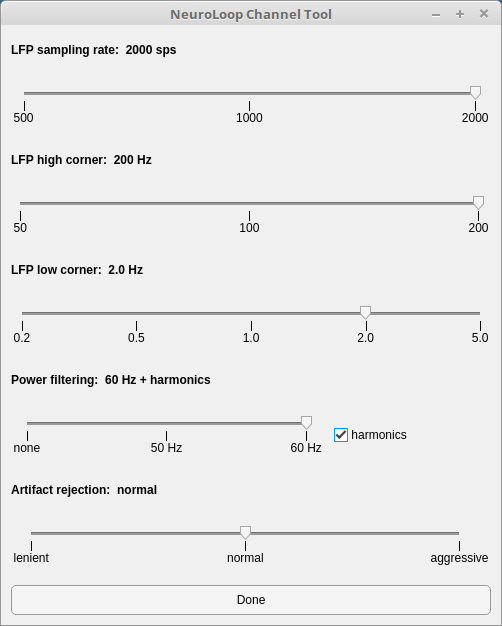
\includegraphics[height=4in]
{screenshots/20201013/gui-2a-procconfig}}
{Processing configuration dialog.}{fig-howto-procconfig}

Artifact rejection is performed first, and then filtering is used to
separate the signal into a spiking component (high frequencies) and a
local field potential component (low frequencies).

Artifact rejection works by looking for large excursions in either the
unfiltered signal itself (typically large voltage transients) or in the
signal's derivative (typically impulse or stepwise changes in the signal).
The artifact rejection slider adjusts how large an excursion has to be in
order to count as an artifact. Artifact regions are removed and interpolated.
Channels that have significant numbers of artifacts are discarded.

Filtering uses infinite impulse response filters that are run forwards and
backwards in time to cancel phase shifts. The LFP filters take about 1 period
of their respective frequencies to stabilize, and the power line notch filter
takes about half a second to stabilize. For best results, set the LFP corner
frequencies a factor of two higher or lower than the highest and lowest
frequencies of interest (respectively), and set the LFP sampling rate ten
times higher than the highest frequency of interest.

Power line filtering has the option of removing the second and third harmonic
of the power line frequency as well as the fundamental frequency. These
frequently appear in recorded signals, but removing them causes filtering to
take considerably longer.

%
%
\clearpage
\section{Processing Dialog}
\label{sect-howto-processing}

When the processing dialog is launched, most controls will be disabled while
processing is happening. The status message at the top of the window shows
the progress of processing (Figure \ref{fig-howto-proc-running}). This will
take a while. When processing is finished, the display updates with graphs
and controls are enabled (Figure \ref{fig-howto-proc-done}).

\figdef{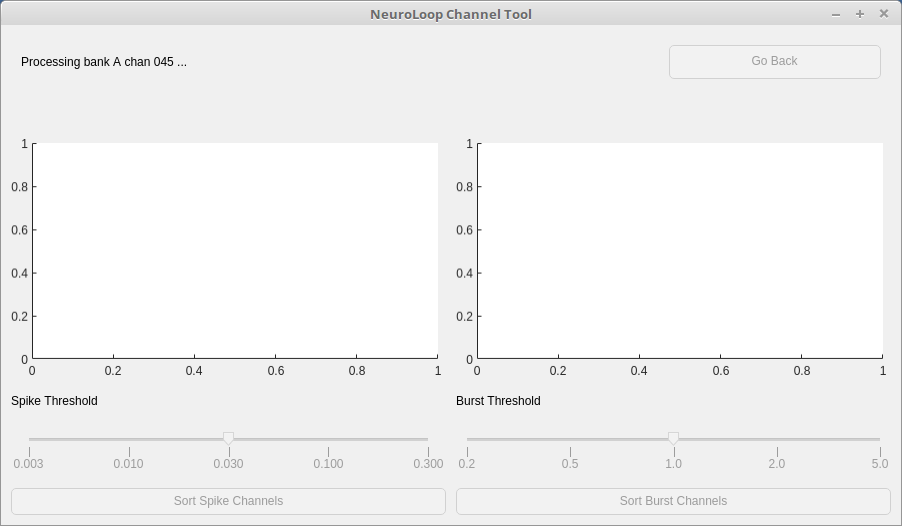
\includegraphics[height=3in]
{screenshots/20201013/gui-3a-process-inprog}}
{Processing dialog while processing is running. Only the status bar is
active.}{fig-howto-proc-running}

\figdef{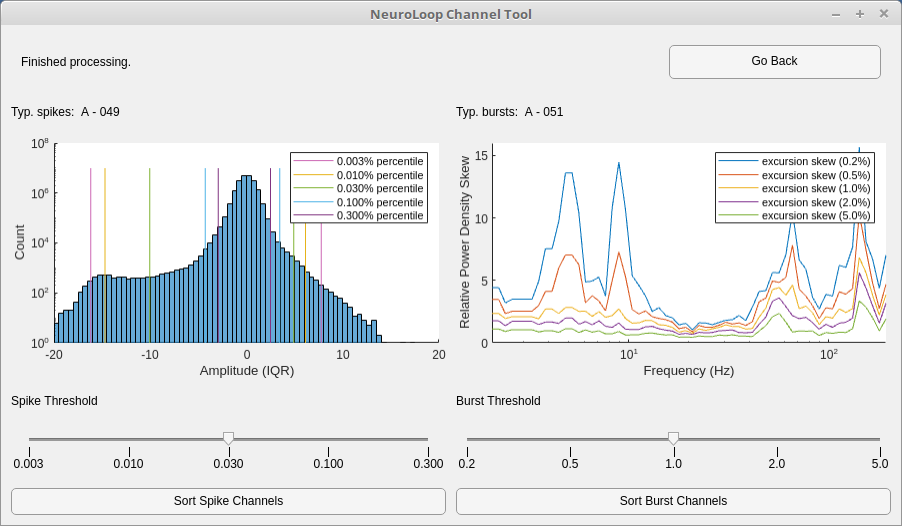
\includegraphics[height=3in]
{screenshots/20201013/gui-3b-process-done}}
{Processing dialog after processing is finished, showing results and
controls.}{fig-howto-proc-done}

Spikes and bursts are identified by looking for negative excursions in
amplitude and positive excursions in the power spectrum, respectively.
``Excursions'' are identified by making a histogram of these respective
quantities and finding where the Nth percentile tails of the probability
distribution are. The ``skew'' is computed by looking at the point half-way
between the tails (the ``midsummary'') and seeing if that is displaced with
respect to the median. Negative skew in the amplitude distribution indicates
spikes, and positive skew in LFP power spectrum frequency bins indicates
transient LFP oscillations (``oscillatory bursts'').

The left graph in Figure \ref{fig-howto-proc-done} shows a histogram of
amplitudes in the high-pass-filtered signal. The tails of the distribution
are asymmetrical, with the plateau indicating significant spiking activity.
The vertical bars indicate where various tail percentiles are. The ``spike
threshold'' slider may be adjusted to select bars where the leftmost bar
intersects the plateau.

The right graph in Figure \ref{fig-howto-proc-done} shows skew in the power
spectrum as a function of frequency. Peaks indicate the presence of
transient LFP oscillations. The different curves use different tail percentile
values. Lower percentile values give greater sensitivity to outlier events.
The ``burst threshold'' slider may be adjusted to pick a curve to use when
identifying channels with oscillatory bursts.

The ``sort spike channels'' button brings up a dialog that ranks channels
by spiking activity, and the ``sort burst channels'' button brings up a
dialog that ranks channels by LFP oscillation activity. These operations are
cheap, so those two dialogs may be entered and left without worry. The
``go back'' button leaves the processing dialog -- discarding the results --
and returns to the data selection dialog.

%
%
\section{Spike Channel Sorting Dialog}
\label{sect-howto-spikes}

\fixme{This dialog is not yet implemented.}

%
%
\section{Burst Channel Sorting Dialog}
\label{sect-howto-bursts}

The burst channel sorting dialog ranks channels by the amount of LFP
transient oscillation activity. This is evaluated by skew in the probability
distribution of power spectrum frequency bin contents over time, per
Section \ref{sect-howto-processing}. On entering the dialog, select a
frequency band using the frequency buttons or sliders, and click ``refresh
list'' to get a ranked list of channels. The result looks like Figure
\ref{fig-howto-bursts-list}.

\figdef{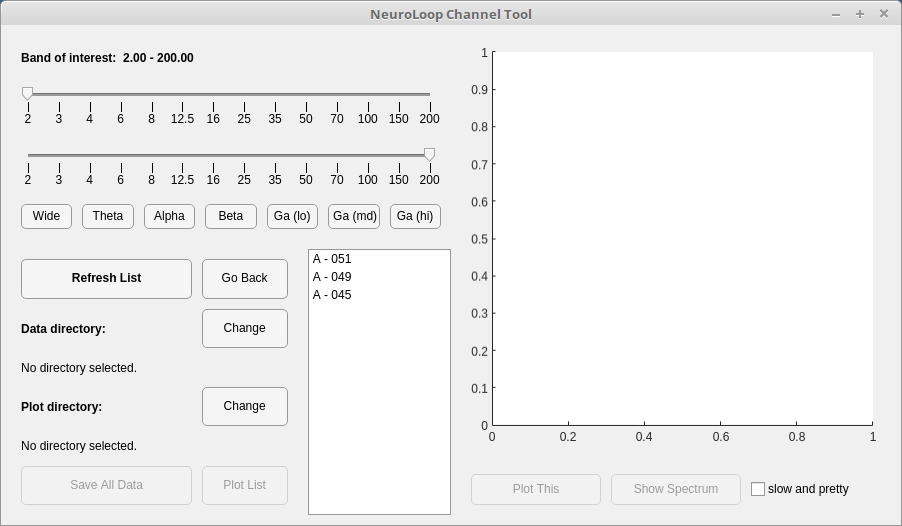
\includegraphics[height=3in]
{screenshots/20201013/gui-4b-burst-refreshed}}
{Burst channel sorting dialog after clicking ``refresh list''.}
{fig-howto-bursts-list}

Channels in the results list are ranked by the amount of in-band skew, with
the channel with the highest amount at the top of the list. To examine the
spectrum of a given channel, click that channel's name in the list. The
plotting area updates to show the amount of skew at each frequency, per
Figure \ref{fig-howto-bursts-skew}. To see excursions overlaid on the power
spectrum, click the ``show spectrum'' button. This gives a plot like the one
shown in Figure \ref{fig-howto-bursts-spect}. To see a persistence spectrum
without skew, click the ``slow and pretty'' checkbox. This gives a plot like
the one in Figure \ref{fig-howto-bursts-persist}. To return to the
excursion plot, click ``Show Excursions''.

\figdef{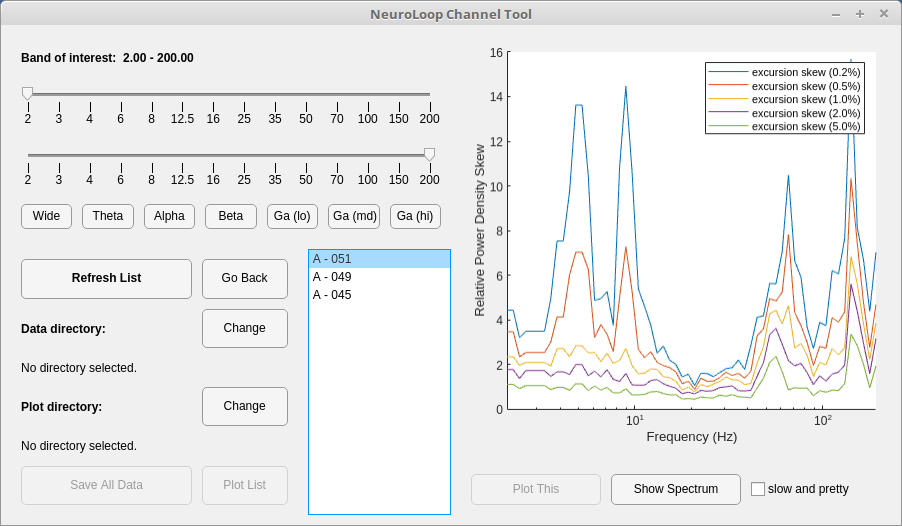
\includegraphics[height=3in]
{screenshots/20201013/gui-4c-burst-chanexcursion}}
{Spectrum skew plot for channel ``A - 051''.}{fig-howto-bursts-skew}

\figdef{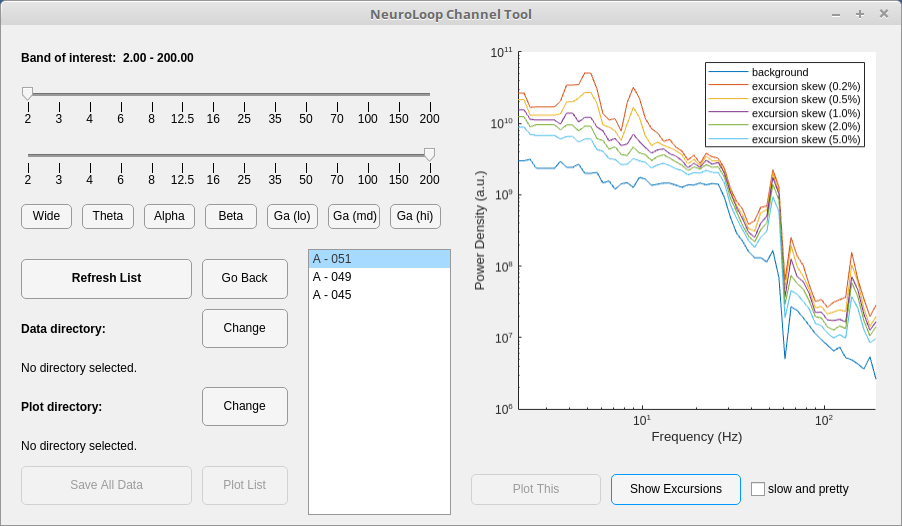
\includegraphics[height=3in]
{screenshots/20201013/gui-4d-burst-chanspect}}
{Power spectrum plot for channel ``A - 051''.}{fig-howto-bursts-spect}

\figdef{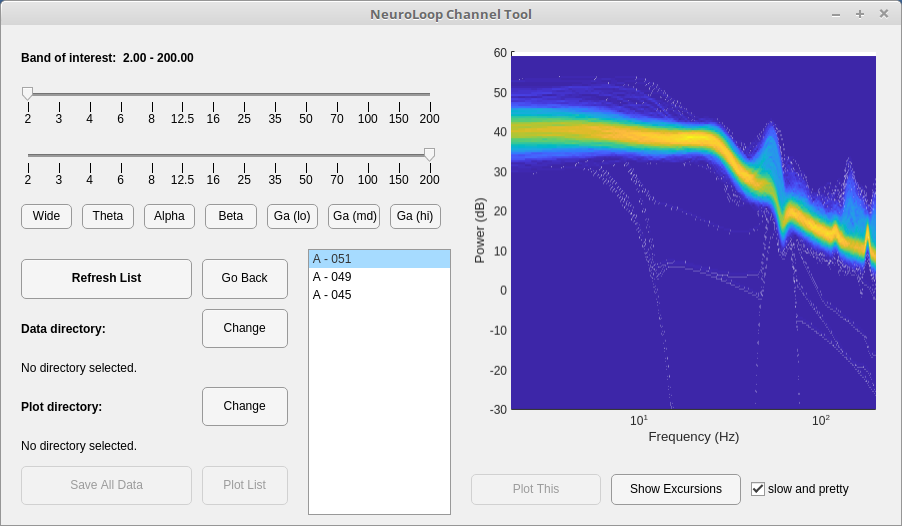
\includegraphics[height=3in]
{screenshots/20201013/gui-4e-burst-chanpersist}}
{Persistence spectrum plot for channel ``A - 051''.}{fig-howto-bursts-persist}

Plots for the selected signal can be saved by clicking the ``plot this''
button after a plot directory has been set. Plots for all channels in the
results list can be generated by clicking the ``plot list'' button. The raw
statistical data used to generate these plots can be saved by clicking ``save
all data'' after a data directory has been set. The ``go back'' button returns
to the processing dialog.

%
% This is the end of the file.

%
%
\end{document}

%
% This is the end of the file.
